\documentclass{standalone}
\usepackage{graphicx}	
\usepackage{amssymb, amsmath}
\usepackage{color}

\usepackage{tikz}
\usetikzlibrary{intersections, backgrounds}
\usepackage{pgfmath}

\definecolor{light}{RGB}{220, 188, 188}
\definecolor{mid}{RGB}{185, 124, 124}
\definecolor{dark}{RGB}{143, 39, 39}
\definecolor{highlight}{RGB}{180, 31, 180}
\definecolor{gray10}{gray}{0.1}
\definecolor{gray20}{gray}{0.2}
\definecolor{gray30}{gray}{0.3}
\definecolor{gray40}{gray}{0.4}
\definecolor{gray60}{gray}{0.6}
\definecolor{gray70}{gray}{0.7}
\definecolor{gray80}{gray}{0.8}
\definecolor{gray90}{gray}{0.9}
\definecolor{gray95}{gray}{0.95}

\begin{document}

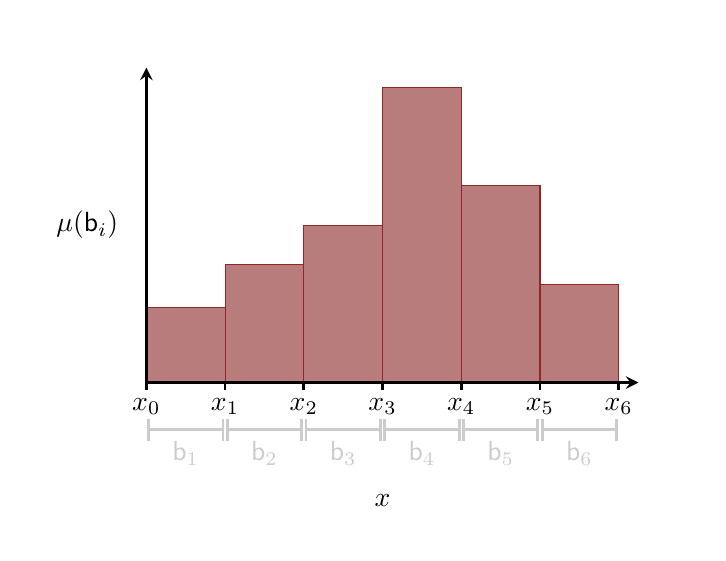
\begin{tikzpicture}[scale=1]
  \draw[white] (-4.5, -3.9) rectangle (4, 2.5);
  
  \foreach [count=\n] \m in {0.95, 1.5, 2, 3.75, 2.5, 1.25} {
    \pgfmathsetmacro{\l}{-3 + 1 * (\n - 1)}
    \pgfmathsetmacro{\u}{-2 + 1 * (\n - 1)}
    \filldraw[fill=mid, draw=dark] (\l, -2) rectangle (\u, \m - 2);
    \draw[gray80, |-|, line width=1] (\l + 0.01, -2.6) -- (\u - 0.01, -2.6);
    \node[gray80] at ({0.5 * (\l + \u)}, -2.9) { $\mathsf{b}_{\n}$ };
  }
    
  \foreach [count=\n] \x in {-3, -2, ..., 3 } {
    \pgfmathtruncatemacro{\nn}{\n - 1}
    \draw[line width=1] (\x, -2) -- (\x, -2.1);
    \node at (\x, -2.3) { $x_{\nn}$ };
  }
  
  \draw[->, >=stealth, line width=1] (-3, -2.0175) -- (-3, +2);
  \draw[->, >=stealth, line width=1] (-3, -2) -- (+3.25, -2);
  \node at (-3.75, 0) { $\mu(\mathsf{b}_{i})$ };
  \node at (0, -3.5) { $x$ };
  
\end{tikzpicture}

\end{document}  